\documentclass[a4paper, notitlepage]{report}
\begin{titlepage}

\begin{center}

%% Insert the TU Delft logo at the bottom of the page.
\begin{tikzpicture}[remember picture,overlay]
    \node at (current page.south)[anchor=south,inner sep=0pt]{
        
\includegraphics{cover/logo}
    };
\end{tikzpicture}

%% Extra whitespace at the top.
\vspace*{2\bigskipamount}

%% Print the title in cyan.
{\makeatletter
\titlestyle\color{tudelft-cyan}\Huge\@title
\makeatother}

%% Print the optional subtitle in black.
{\makeatletter
\ifx\@subtitle\undefined\else
    \bigskip
    \titlefont\titleshape\LARGE\@subtitle
\fi
\makeatother}

\bigskip
\bigskip

by
%door

\bigskip
\bigskip

%% Print the name of the author.
{\makeatletter
\titlefont\Large\bfseries\@author
\makeatother}

\vfill

in partial fulfillment of the requirements for the degree of
%in overeenstemming met de vereisten voor het verkrijgen van de graad van

\bigskip
\bigskip

{\bfseries Master of Science}

in Applied Physics

\bigskip
\bigskip

at the Delft University of Technology,
%aan de Technische Universiteit Delft,

to be defended publicly on Tuesday January 1, 2013 at 10:00 AM.
%in het openbaar de verdedigen op dinsdag 1 januari om 10:00 uur.

\vfill

\begin{tabular}{lll}
%% Add additional information here, per faculty requirements, e.g
%    Student number: & 1234567 \\
%    Project duration: & \multicolumn{2}{l}{March 1, 2012 -- January 1, 2013} \\
    Supervisor: & Prof.\ dr.\ ir.\ A.\ Einstein \\
    Thesis committee:
        & Prof.\ dr.\ C.\ F.\ Xavier, & TU Delft \\
        & Dr.\ E.\ L.\ Brown, & TU Delft \\
        & Ir.\ M.\ Scott, & Acme Corporation
\end{tabular}

%% Only include the following lines if confidentiality is applicable.
\bigskip
\bigskip
\emph{This thesis is confidential and cannot be made public until December 31, 2013.}
%\emph{Op dit verslag is geheimhouding van toepassing tot en met 31 december 2013.}

\bigskip
\bigskip
An electronic version of this thesis is available at \url{http://repository.tudelft.nl/}.
%Een elektronische versie van dit verslag is beschikbaar op \url{http://repository.tudelft.nl/}.

\end{center}

\end{titlepage}


% All imports needed for file

% General
\usepackage[a4paper,top=1.25in,right=1in,bottom=1.25in,left=1in]{geometry}
\usepackage[utf8]{inputenc}
\usepackage[T1]{fontenc}
\usepackage{textcomp}
\usepackage[bitstream-charter]{mathdesign}
\usepackage{cite}

\usepackage{import}
\usepackage{standalone}
\usepackage{epstopdf}



% Math
\usepackage{amsmath}	% some standard math functions
%\usepackage{amssymb}	% more mathematical symbols
\usepackage{amsbsy}	% enable bold mathematics
\usepackage{bm}
%\usepackage{amsthm}	% enable theorem statements
\usepackage{trfsigns} 	% symbols for transforms

% Text formatting
\usepackage{fancyhdr}	% allow more control over page headers/footers
\usepackage{enumitem}	% allow control over enumerate, itemize, description
\usepackage{setspace}	% allow control over spacing
\usepackage{lastpage}	% provide label for last page in document
\usepackage{sectsty}	% allow control over section styling
\usepackage{url}

% Floats
\usepackage{xcolor}		% enable use of colors
\usepackage{graphicx}		% enable graphics
\usepackage{float}		% enable floats
\usepackage[section]{placeins}	% prevent floats from moving past e.g. sections
\usepackage[small, bf, hang, figurename=Fig.]{caption}	% enable captions for floats (images etc.)
\captionsetup{width=.8\textwidth} % captions not too wide
\usepackage{subcaption}		% enable subcaptions for floats (images etc.)
\usepackage[nottoc]{tocbibind}		% put more stuff in TOC

% Styling data
\pagestyle{fancyplain}

% Title page
\makeatletter
\let\inserttitle\@title
\makeatother

% Page header
\setlength{\headwidth}{\textwidth}
\lhead{} % leave left header empty
\chead{}
\rhead{} % leave right header empty
\lfoot{} % leave left footer empty
\cfoot{} % leave center footer empty
\rfoot{}
\renewcommand{\headrulewidth}{0.3pt}
\renewcommand{\footrulewidth}{0pt}

% Section, equation and figure numbering
\usepackage{chngcntr} 
\counterwithout{figure}{chapter}
\renewcommand{\thechapter}{\Roman{chapter}}
\renewcommand{\thesection}{\Roman{chapter}.\arabic{section}}
\renewcommand{\thesubsection}{\Roman{chapter}.\arabic{section}.\arabic{subsection}}
\renewcommand{\thesubsubsection}{\alph{subsubsection})}
\renewcommand{\thefigure}{\arabic{figure}}
\renewcommand{\thesubfigure}{\alph{subfigure}}
\renewcommand{\theequation}{\thechapter--\arabic{equation}}
\setcounter{tocdepth}{1}
\captionsetup[figure]{labelsep=period}

% Nice enumerations
\newlist{enum}{enumerate}{1}
\setlist[enum]{label=\textbf{[\arabic*]}} % \arabic or \alpha
\setlist{itemsep=-5pt}

% Nice \begin{StateDescription} for FSM descriptions
\newlist{StateDescription}{description}{1}
\setlist[StateDescription]{font=\normalfont\scshape, labelwidth=12em, leftmargin=12em,listparindent=0em,itemindent=0em}

% Section formatting
\definecolor{title-gray}{gray}{0.45}		% grijstint voor headers
\renewcommand*\sfdefault{lmss}
\allsectionsfont{\sffamily\color{title-gray}}	% sans-serif in headers

% Page layout
\onehalfspacing					% Wide margins for text
\usepackage{chngpage}			% customize margins of certain pages
\usepackage{adjustbox}

% Text macros
\usepackage{xspace}
\newcommand{\matlab}{MATLAB\xspace}		% fancy MATLAB command
\newcommand{\norm}[1]{\left\lVert#1\right\rVert}% Command for vector norm
\newcommand{\abs}[1]{\left\lvert#1\right\rvert}% Command for abs
\newcommand{\todo}[1]{\textbf{\textcolor{red}{#1}}}	% placeholder stuff
\let\oldhat\hat
\renewcommand{\vec}[1]{\bm{#1}} % bold vectors in math mode
\newcommand{\vechat}[1]{\oldhat{\bm{#1}}} % hat in vector mode
\newcommand{\mat}[1]{\bm{#1}} % bold matrix in math mode

%links
\usepackage{hyperref}
\hypersetup{ %setup hyperlinks
    colorlinks=true,
    citecolor=black,
    filecolor=black,
    linkcolor=black,
    urlcolor=black
}

\begin{document}

\section{SRO characterization}
\label{sec:sro-characterization}
An attempt has been made to characterize the degree of sampling rate offset in the used smartphones. Based on the literature (see section \ref{sec:problem-sro}), it is expected that the offset is quite low compared to the used sampling rate. Therefore, this work has focused on providing quantitative measurements of sample rate offset. Implementation and comparison of correction algorithms was left as a topic of future research. 

\subsection{Measurement setup}
In order to measure SRO, the anechoic chamber at the Delft University of Technology was set up with three identical Nexus 5 smartphones streaming audio to a computer at a nominal sampling frequency of $48~\mathrm{kHz}$. The audio source consisted of a loudspeaker connected to a high-fidelity audio interface, RME Fireface 800. The measurement setup is depicted in Fig.~\ref{fig:sro_measurement_setup} and a picture of the actual setup is shown in Fig.~\ref{fig:sro_measurement_picture}.

The audio interface produced an hour-long continuous sine waveform of $15~\mathrm{kHz}$ which was recorded by the smartphones and sent to the computer, with the intent of computing the sample rate offset from the ideal $48~\mathrm{kHz}$ value.

As will become clear in the next section, this offset is detect when a higher-frequency sine wave is used. However, if the frequency is chosen too high, the response of the microphone is no longer adequate for receiving the signal. Therefore, $15~\mathrm{kHz}$ was chosen to strike a balance between high frequency and and good microphone gain. The microphone response was taken from the results of Gaubitch, Martinez, Kleijn and Heusdens \cite{Gaubitch2014} and preliminary results from Brinkman and De Rooij \cite{BAP:RosalieTim} for Nexus 5 microphone directivities.

\begin{figure}[hbt]
	\centering
		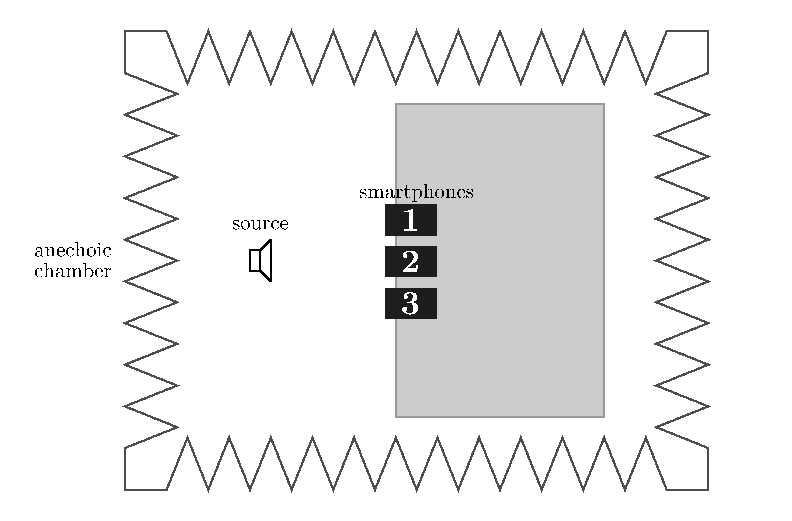
\includegraphics[width=0.8\textwidth]{figures/sro-measurement/measurement_setup}
		\caption[Measurement setup used for SRO measurements.]{Schematic representation of the measurement setup used for SRO measurements. The figure shows the anechoic chamber at the Delft University of Technology with three smartphones and a loudspeaker. Not depicted: computer connected via Wi-Fi to receive the sent audio signals.}
		\label{fig:sro_measurement_setup}
\end{figure}

\begin{figure}[bht]
	\centering
		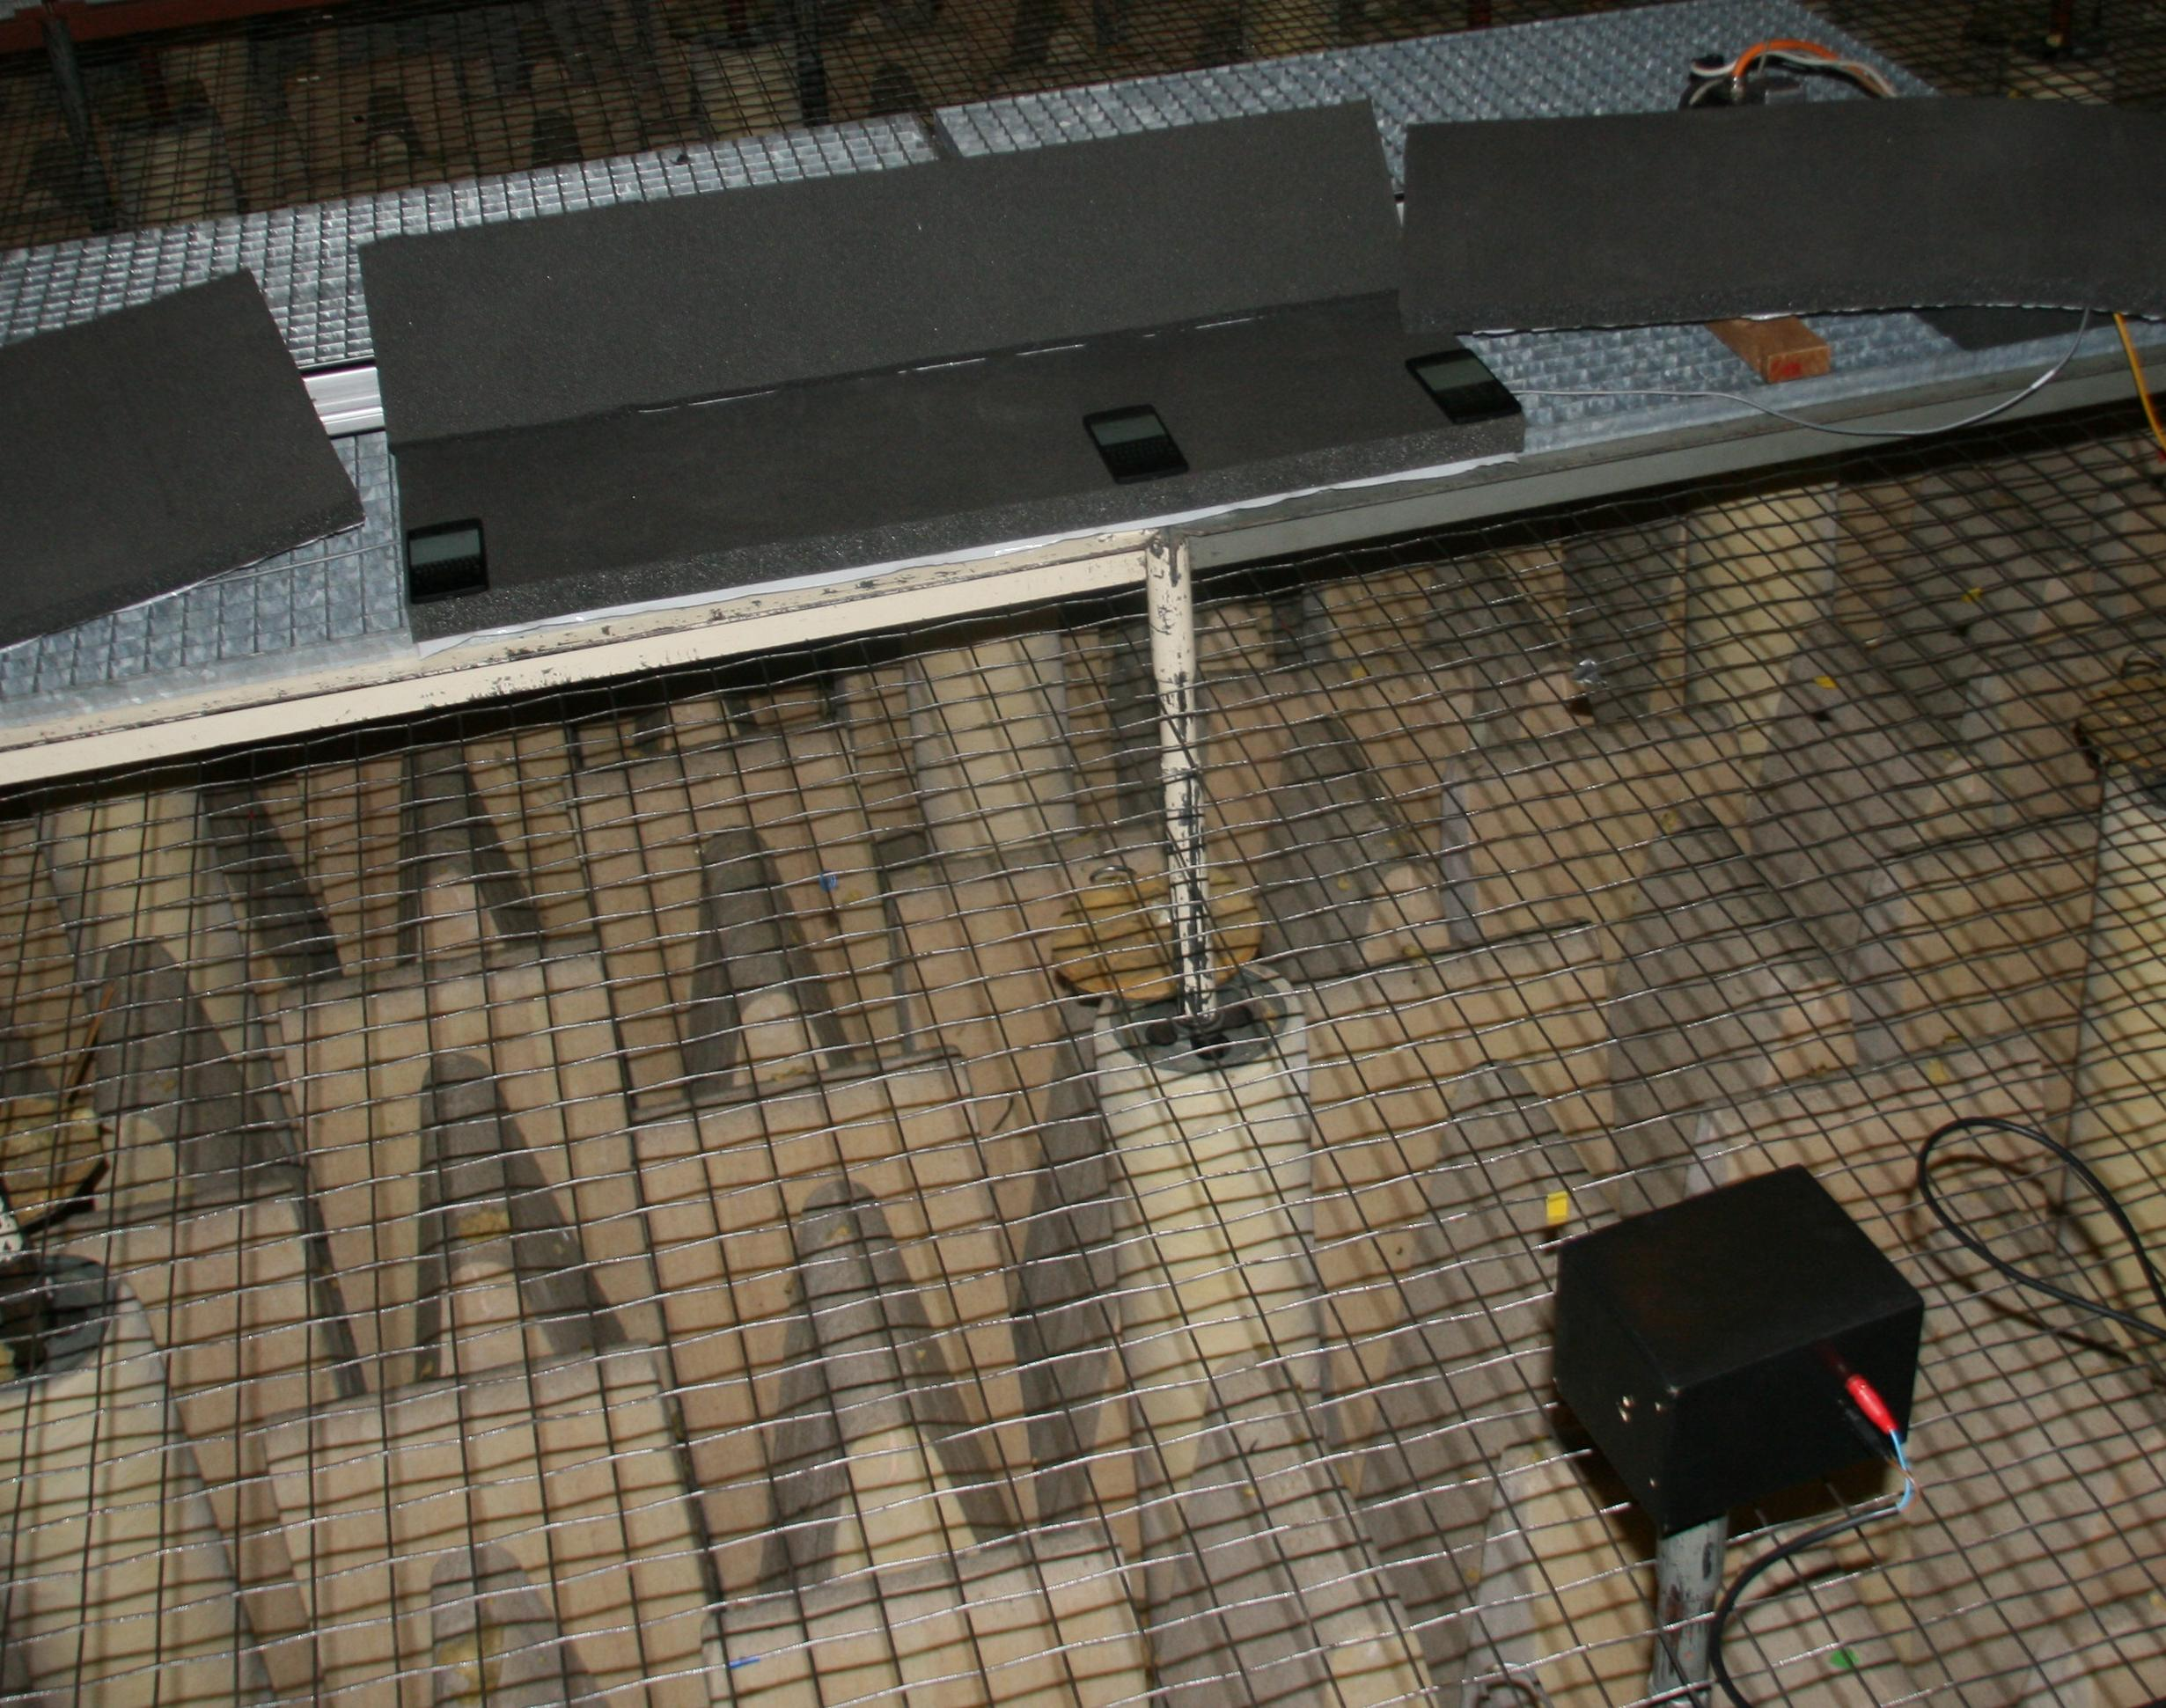
\includegraphics[width=0.8\textwidth]{figures/sro-measurement/measurement_picture}
		\caption[SRO measurement setup in the anechoic chamber.]{An actual picture of the setup in the anechoic chamber. The three phones are resting on a piece of foam in the top half of the image, with the speaker visible in the lower right.}
		\label{fig:sro_measurement_picture}
\end{figure}

\subsection{SRO estimation}
The resolution at which the frequency can be estimated can be calculated from the properties of the discrete Fourier transform (DFT). Let $N$ be the number of time-domain samples in the series $\vec{s}[t]~,t\in\{0,1,\dots N-1\}$. The DFT is then the frequency-domain representation of the periodically extended discrete-time signal $\vec{s}[t]$, and is given by $\vec{S}[2\pi k/N],~k\in\{0, 1\dots N-1\}$. Thus, we also have $N$ samples in the frequency domain \cite[p.~421-422]{Proakis2007}.
Recalling that the DFT consists of frequencies from $-f_s/2$ to $f_s/2$ (assuming the time-domain signal was bandlimited below $f_s/2$), the frequency resolution can be calculated from $\Delta f=f_s/N$. But since $N=Tf_s$, $\Delta f = 1/T$ where $T$ represents the duration in seconds of the sampled signal $s[t]$.

It can be seen that a short DFT window provides fine time resolution but coarse frequency resolution, and conversely a long DFT window provides fine-grained time resolution at the expense of coarse frequency resolution. Put differently, a long DFT window provides more detailed information about the frequencies present in a signal, but provides less detail about \emph{when} these frequencies are present in time.

For these experiments, a sampling rate of $48~\mathrm{kHz}$ was chosen as this is the highest widely supported sampling rate on Android smartphones. Window lengths varying from $5~\mathrm{minutes}$ ($\Delta f = 3.3~\mathrm{mHz}$) to $30~\mathrm{seconds}$ ($\Delta f = 33~\mathrm{mHz}$) were chosen for performing the DFT.


Once the recorded frequency is known, the SRO can be determined:
$$\text{SRO} = \frac{\left(f_{\text{play}}-f_{\text{detected}}\right)\cdot f_s}{f_\text{play}}$$
where $f_{\text{play}}, f_{\text{detected}}, f_{\text{s}}$ indicate played audio frequency, detected audio frequency from the recording and sampling frequency, respectively.

\subsection{Results}
The SRO for these smartphones is lower than predicted by the literature, in the order of $0.2~\mathrm{Hz}$ (Fig.~\ref{fig:sro_result}) and does not change rapidly with time. Full DFT plots for all window lengths may be found in Fig.~\ref{app:sro_total} in appendix \ref{app:results} and a discussion of the results in section \ref{sec:disc_sro}.

\begin{figure}[htb]
\begin{adjustwidth}{-1in}{-1in}
\centering
	\begin{subfigure}{0.5\textwidth}
		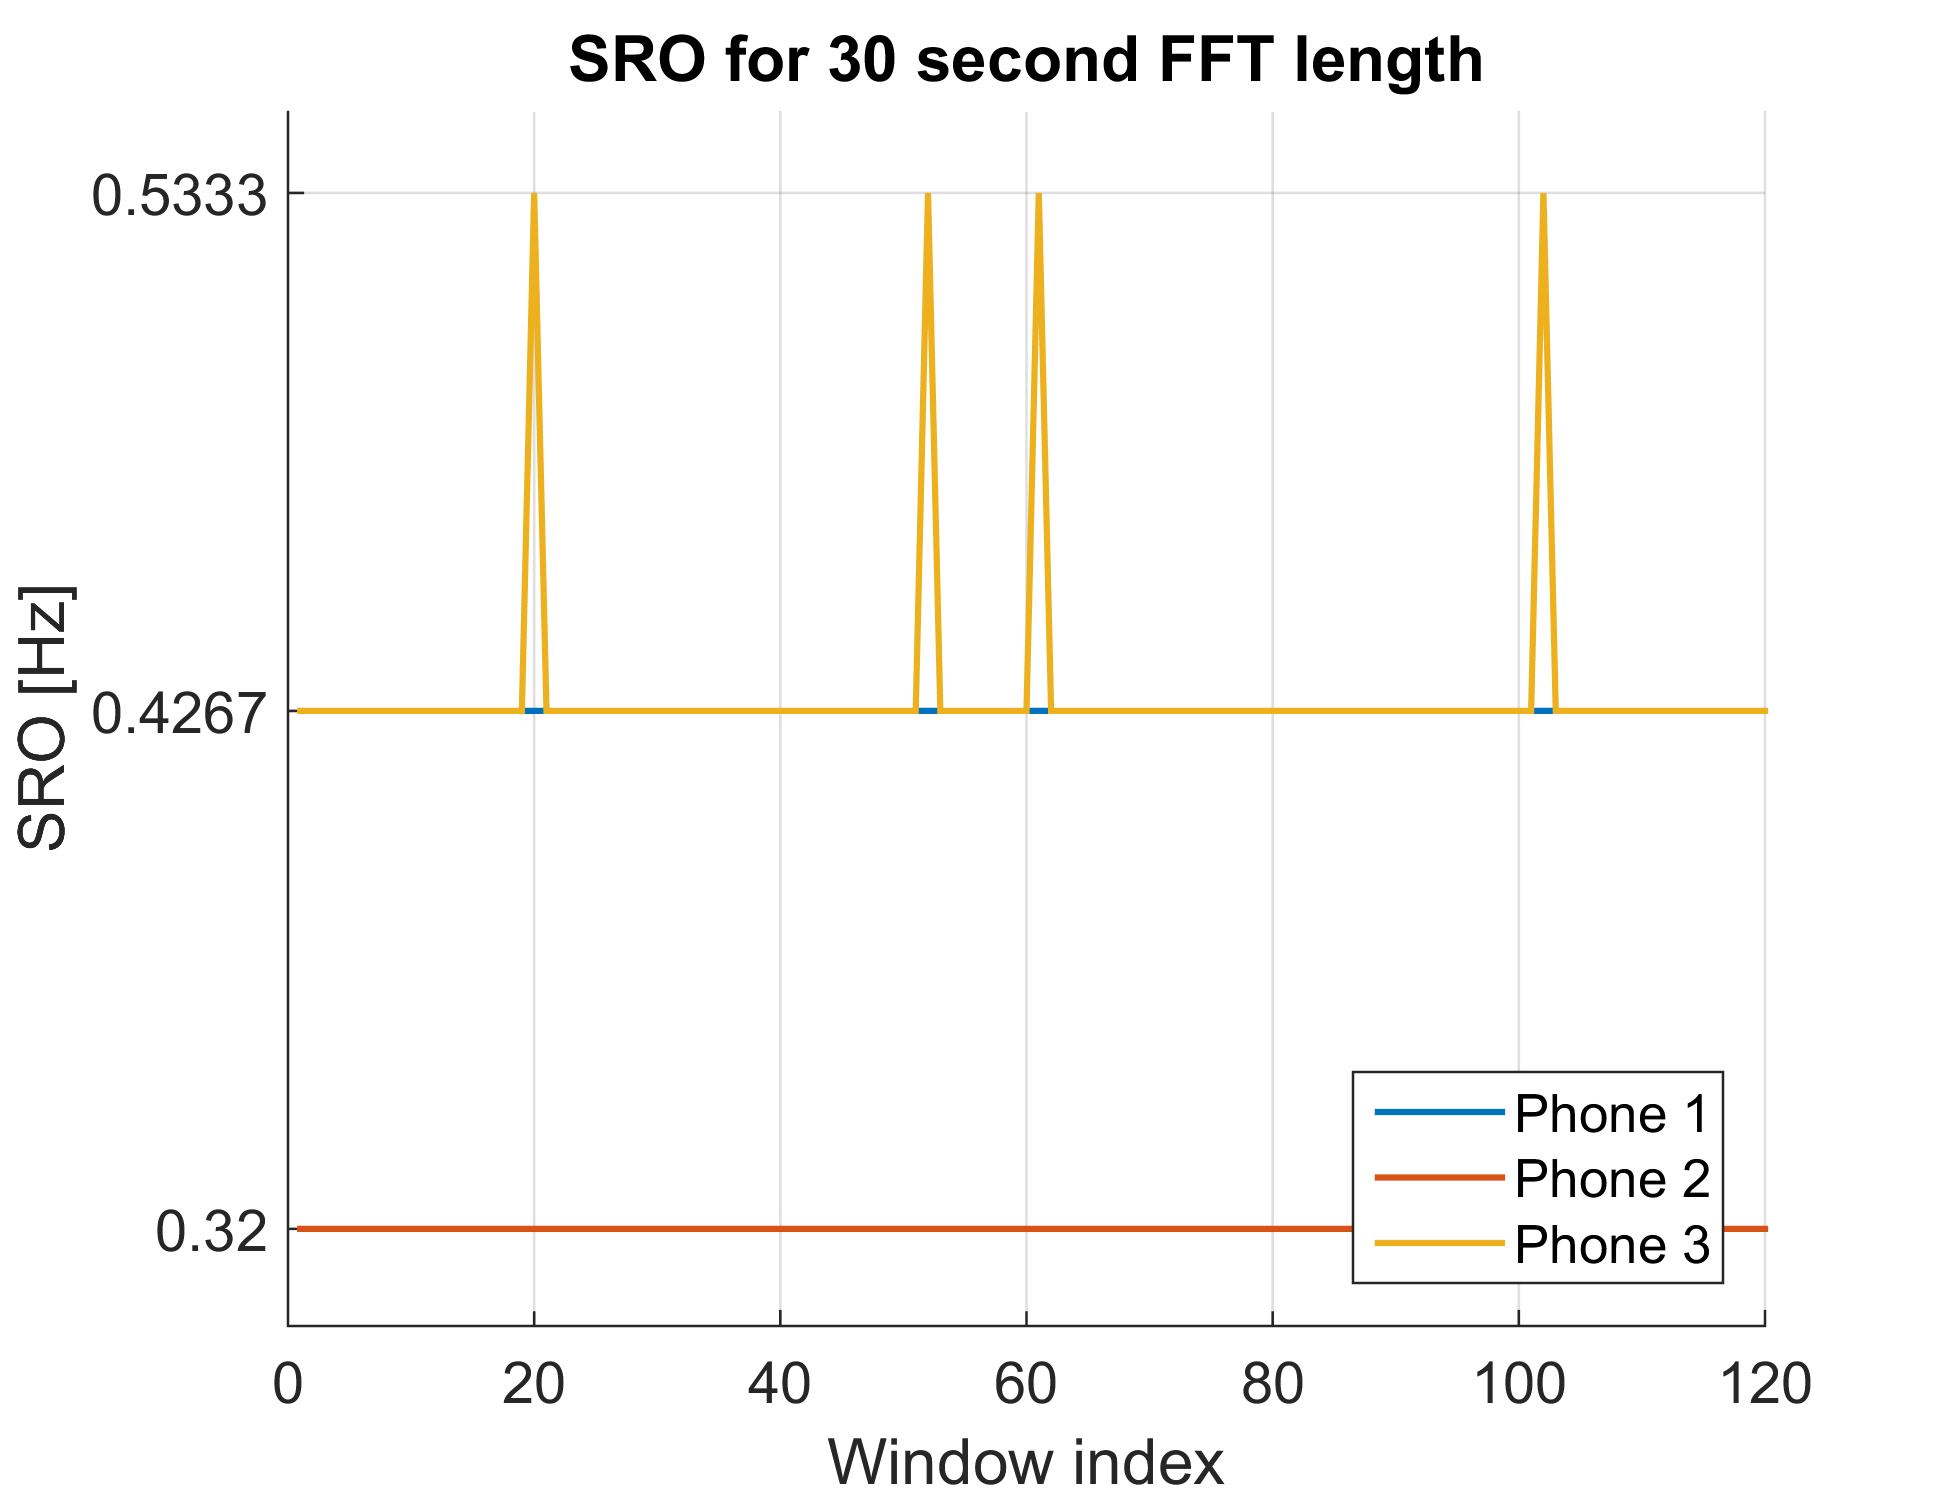
\includegraphics[width=\textwidth]{figures/sro-measurement/sro-30sec}
		\caption{30 second DFT window, $\Delta f=33~\mathrm{mHz}$.}
		\label{fig:sro_30sec}
	\end{subfigure}
	\begin{subfigure}{0.5\textwidth}
		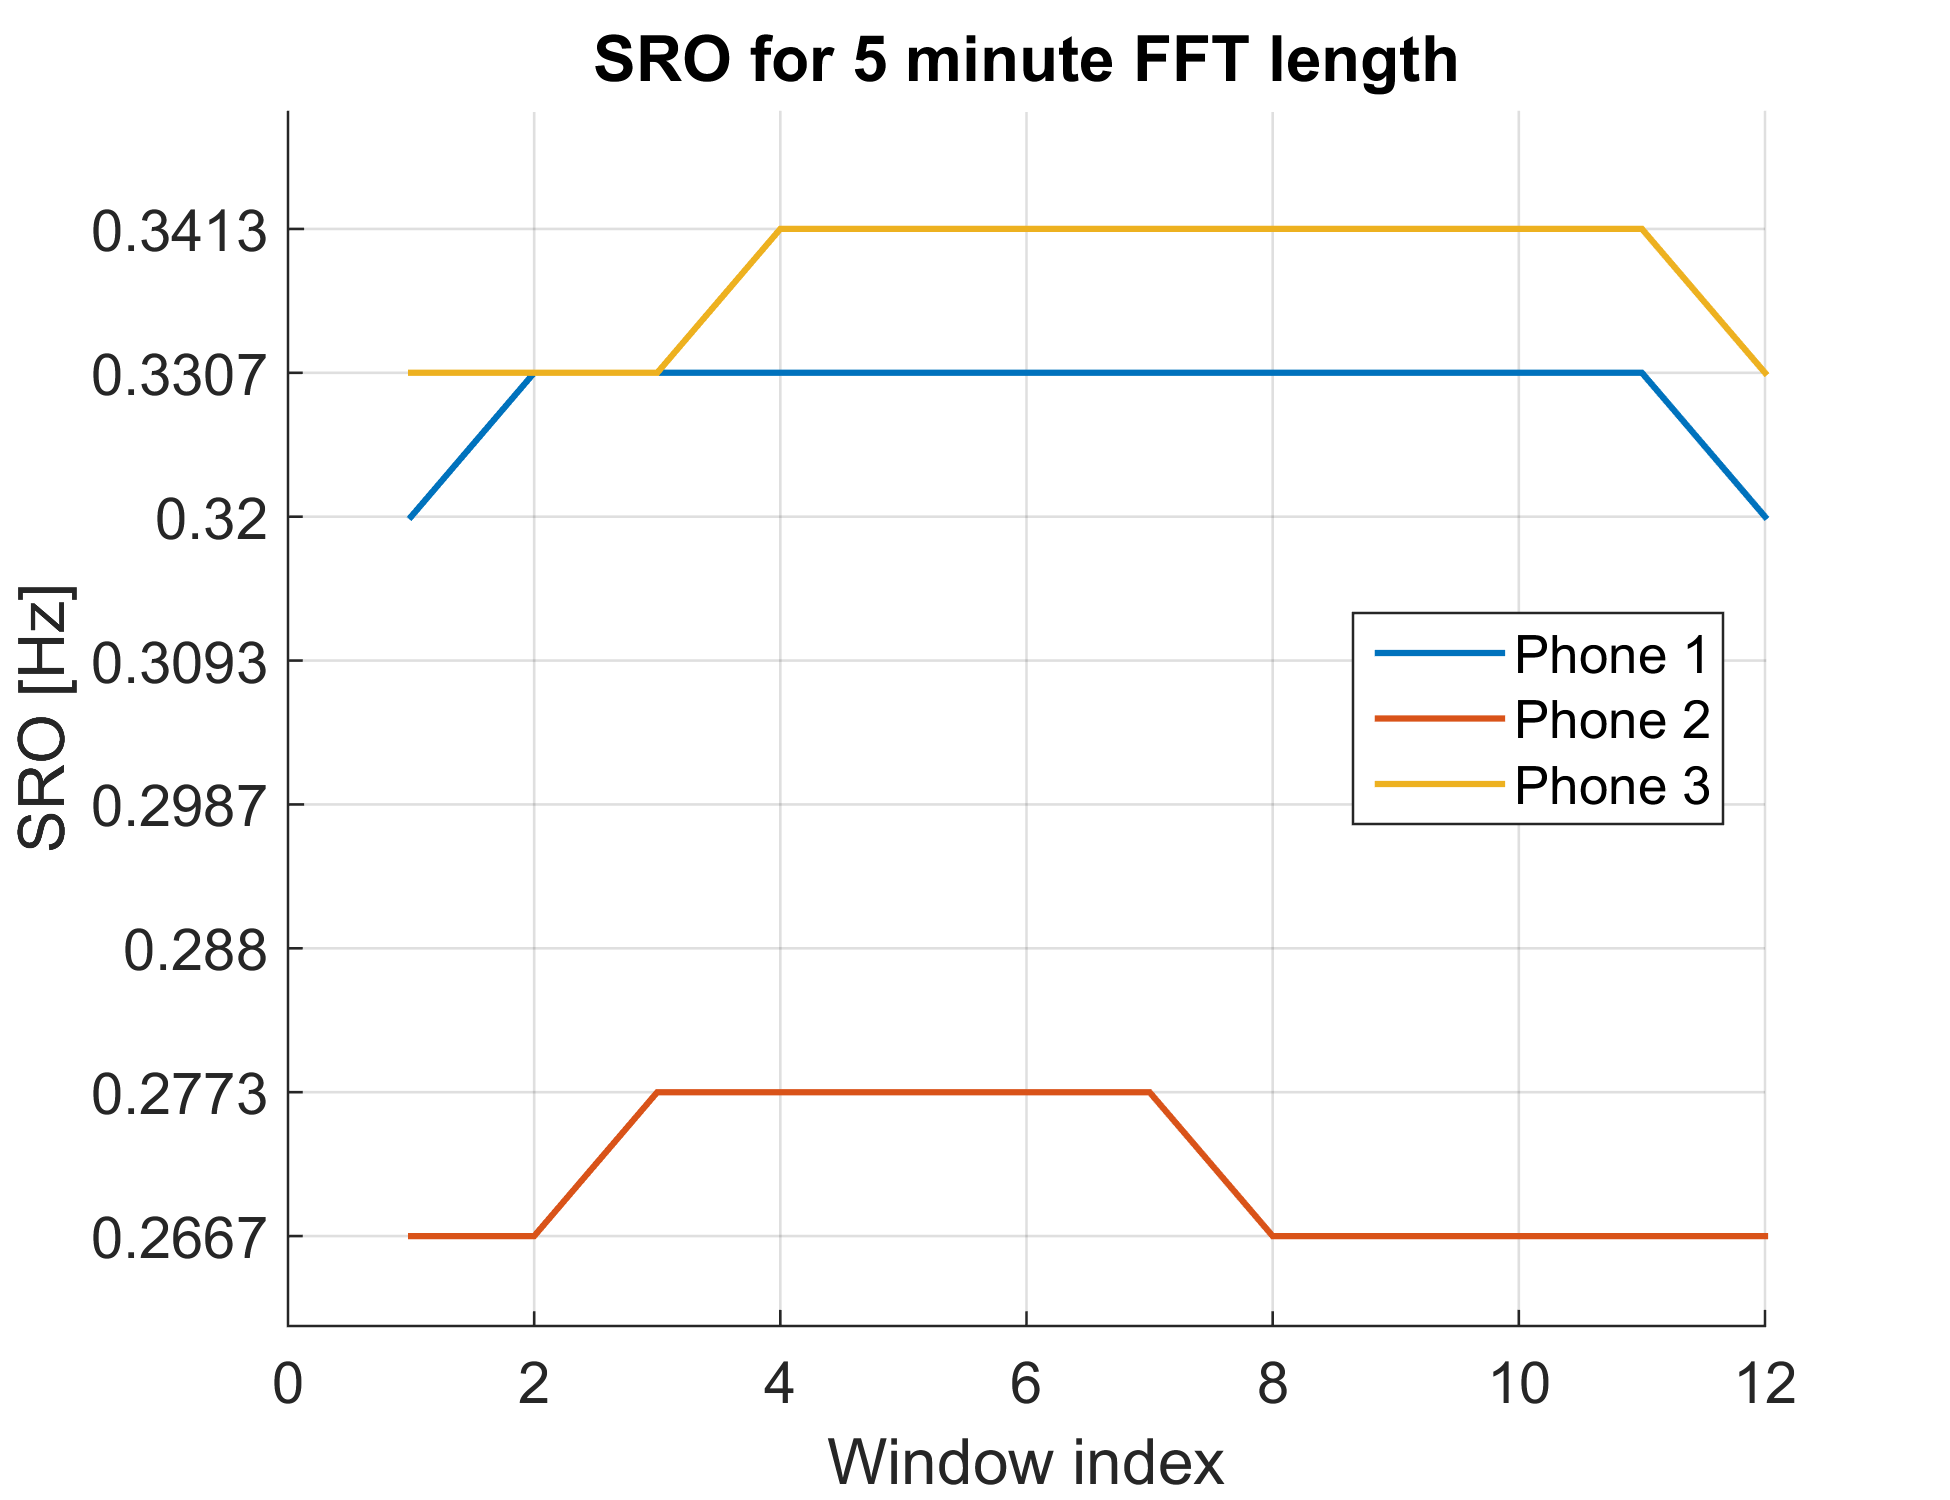
\includegraphics[width=\textwidth]{figures/sro-measurement/sro-5min}
		\caption{Five minute DFT window, $\Delta f=3.3~\mathrm{mHz}$}
		\label{fig:sro_5min}
	\end{subfigure}	
\end{adjustwidth}
\caption[SRO measurement result.]{Sampling rate offset measurements for two DFT window lengths. A larger DFT window gives a higher frequency resolution $\Delta f$ but lower time resolution.}
\label{fig:sro_result}
\end{figure}
\end{document}
